\documentclass[11pt]{article}

\marginparwidth 0.5in
\oddsidemargin 0.25in
\evensidemargin 0.25in
\marginparsep 0.25in
\topmargin 0.25in
\textwidth 6in
\textheight 8in

\usepackage{amsmath, amssymb}
\usepackage{upgreek}
\usepackage{latexsym}
\usepackage{graphicx}

\begin{document}
\begin{flushleft}
Juan Miguel C. Manalo \\
2014-40093 \\
CS 145 THWMXY-HONOR
\end{flushleft}

\begin{center}
\textbf{CS145 Lab Exercise 3: Wireshark Lab - Internet Protocol and Traceroute Operation}
\end{center}

\begin{enumerate}
\item
9 routers, not including the server hosting the Philippine Daily Inquirer.
\begin{center}
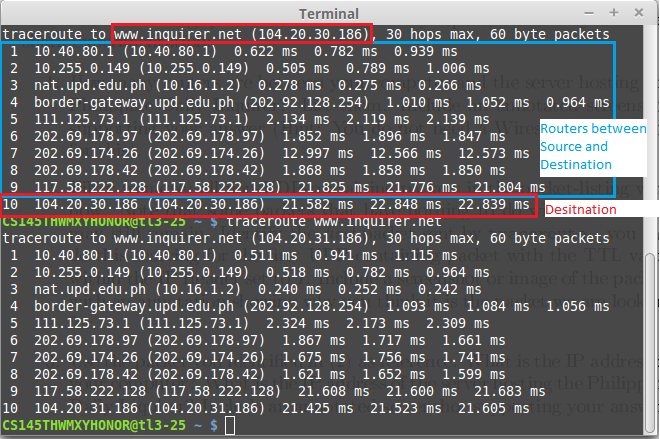
\includegraphics[scale=0.5]{Q1}
\end{center}

\item
Packet \#7
\begin{center}
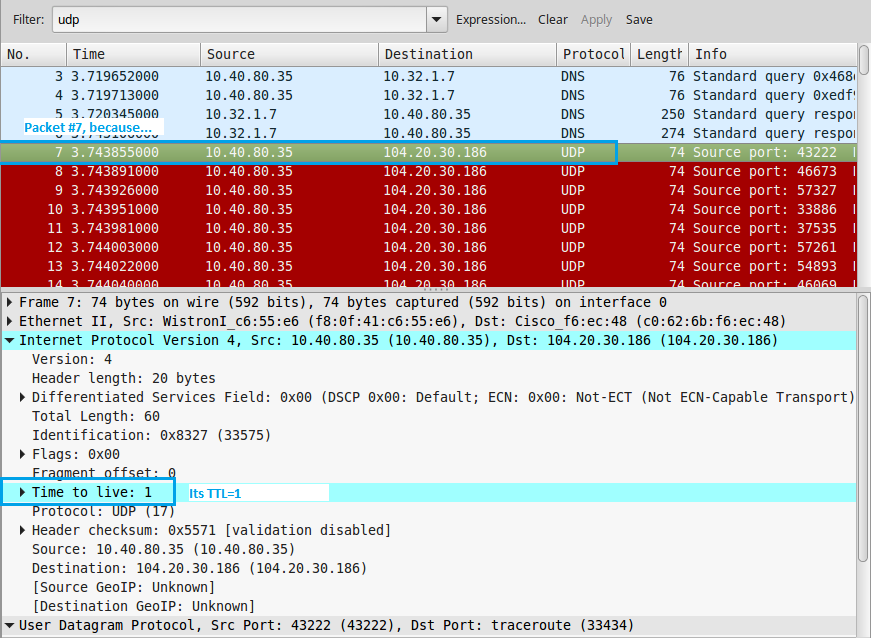
\includegraphics[scale=0.4]{Q2}
\end{center}

\item
IP Address (Computer): \textbf{10.40.80.35} \\
IP Address (Website): \textbf{104.20.30.186}
\begin{center}
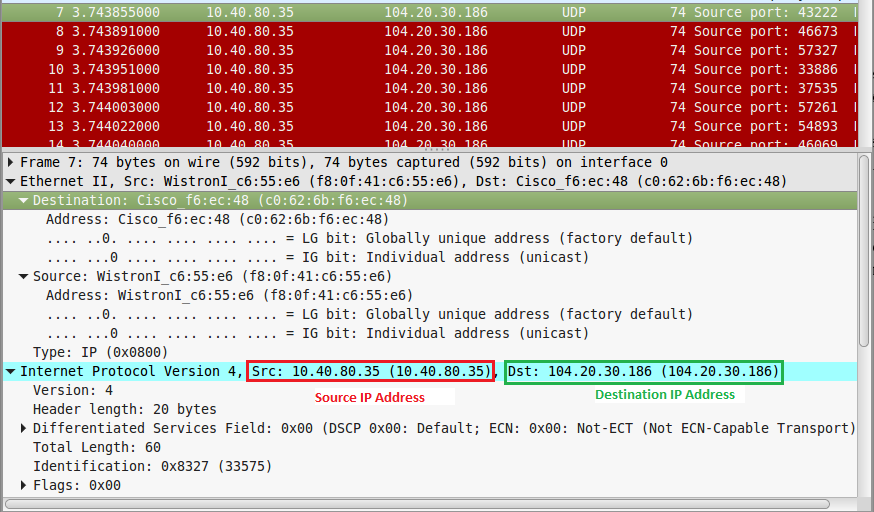
\includegraphics[scale=0.4]{Q3}
\end{center}

\item
IP Header: \textbf{20 bytes} \\
IP Datagram Payload: \textbf{40 bytes} \\
As annotated, the total length of the IP Datagram is 60 bytes. To get the payload, subtract the IP Header bytes from the total length of the datagram. Hence, $60 - 20 = 40$ bytes.
\begin{center}
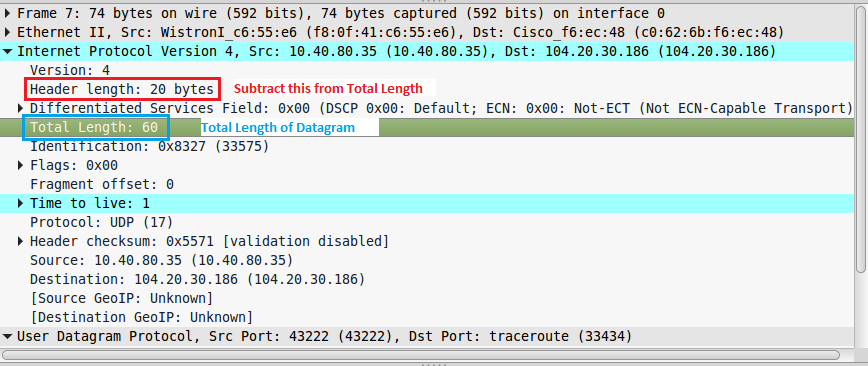
\includegraphics[scale=0.4]{Q4}
\end{center}

\item
The Identification and the Checksum. They are as follows:
\begin{itemize}
\item{Packet \#7: 0x8327 (Identification), 0x5571 (Checksum)}
\item{Packet \#8: 0x8328 (Identification), 0x5570 (Checksum)}
\item{Packet \#9: 0x8329 (Identification), 0x556f (Checksum)}
\end{itemize}

\item
The Internet Protocol Version, Header Length, Differentiated Services Field, Flags, TTL, Protocol, Source, and Destination.

\item
The values in the Identification field increase by 1 each succeeding packet.

\item
Traceroute does not assume that the ICMP messages will arrive in order. It depends on the delay time of each UDP packet. An ICMP message is associated to its corresponding UDP packet through the Source and Destination Ports in the UDP header.
\begin{center}
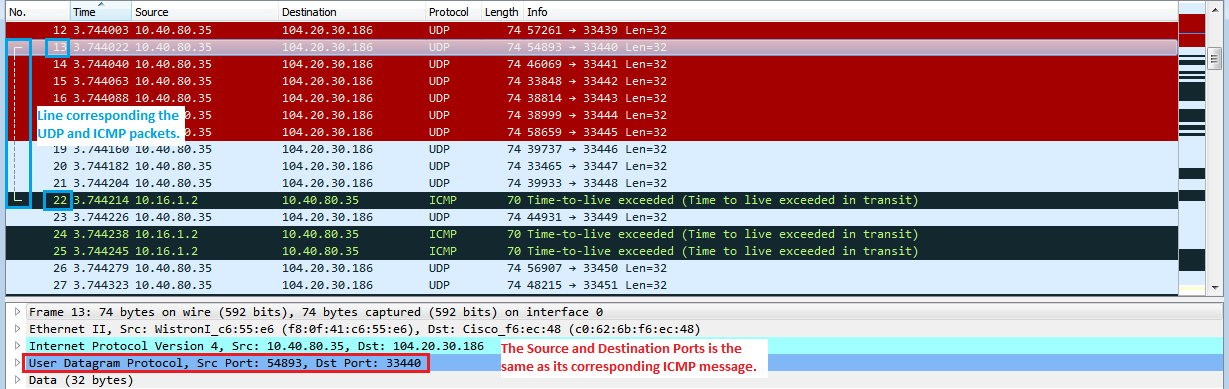
\includegraphics[scale=0.5]{Q8}
\end{center}

\item
Packet \#22 (caused by Packet \#13)
\begin{center}
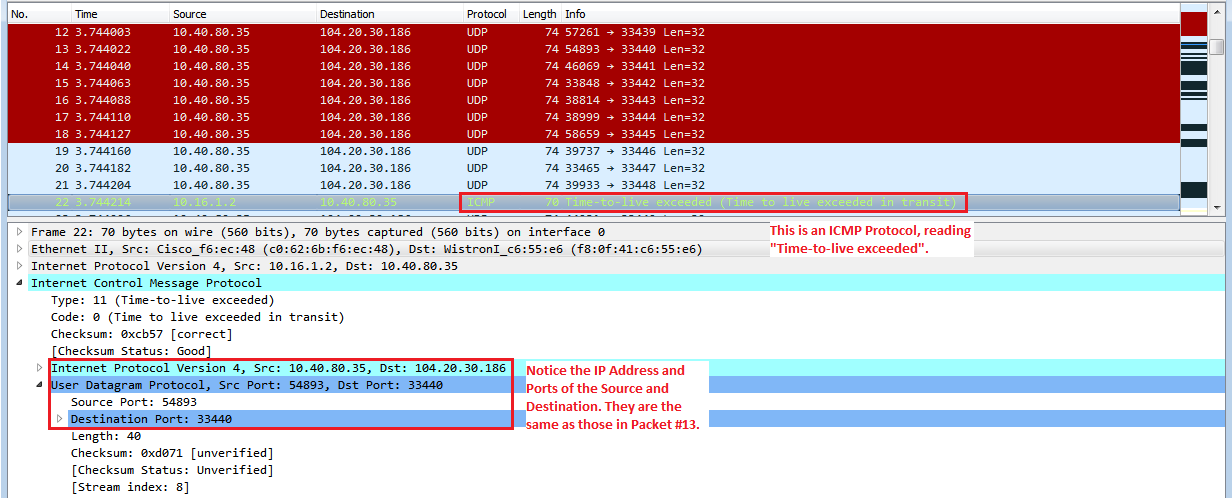
\includegraphics[scale=0.5]{Q9A} \\
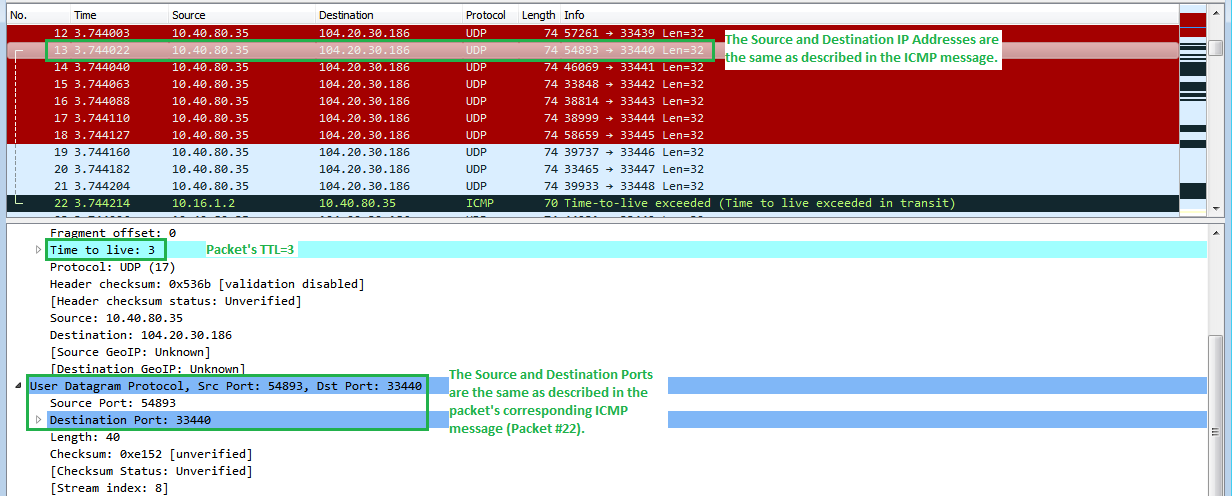
\includegraphics[scale=0.5]{Q9B}
\end{center}

\item
Timestamp Delays:
\begin{itemize}
\item{UDP1 = 3.744214 s - 3.744022 s = 192 ms}
\item{UDP2 = 3.744238 s - 3.744040 s = 198 ms}
\item{UDP3 = 3.744245 s - 3.744063 s = 182 ms}
\end{itemize}

Delay based on Traceroute Values:
\begin{center}
\begin{tabular}{|c|c|c|c|}
\hline
\textbf{\#} & \textbf{UDP1} & \textbf{UDP2} & \textbf{UDP3} \\
\hline
1 & 0.622 ms & 0.782 ms & 0.939 ms \\
\hline
2 & 0.505 ms & 0.789 ms & 1.006 ms \\
\hline
3 & 0.278 ms & 0.275 ms & 0.266 ms \\
\hline
4 & 1.010 ms & 1.052 ms & 0.964 ms \\
\hline
5 & 2.134 ms & 2.119 ms & 2.139 ms \\
\hline
6 & 1.852 ms & 1.896 ms & 1.847 ms \\
\hline
7 & 12.997 ms & 12.566 ms & 12.573 ms \\
\hline
8 & 1.868 ms & 1.858 ms & 1.850 ms \\
\hline
9 & 21.825 ms & 21.776 ms & 21.804 ms \\
\hline
10 & 21.582 ms & 22.848 ms & 22.839 ms \\
\hline
\textbf{Total} & 64.673 ms & 65.961 ms & 66.281 ms \\
\hline
\textbf{\textbf{X Hops (3)}} & 194.02 ms & 197.88 ms & 198.84 ms \\
\hline
\end{tabular}
\end{center}

\begin{center}
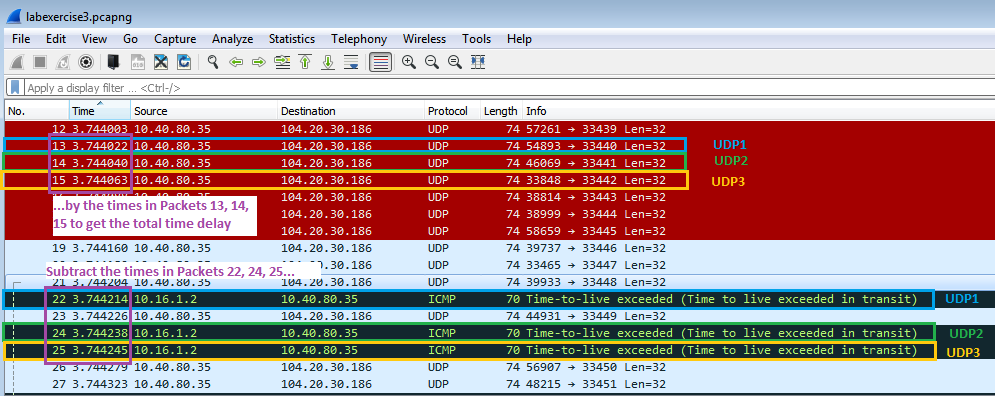
\includegraphics[scale=0.5]{Q10A} \\
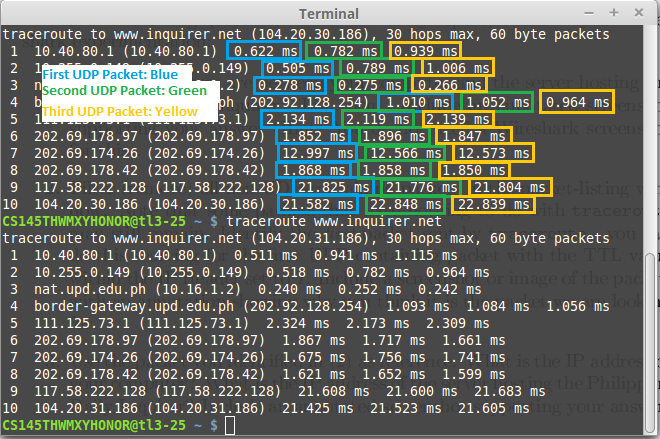
\includegraphics[scale=0.5]{Q10B}
\end{center}

\end{enumerate}

\end{document}